%!TEX root = ../Diploma.tex


\begin{section}{Описание методологии}
   В этой главе будет дано описание начального набора данных,
   его предобработка, признаки, которые были использованы для построения классификатора, а также описание использовавшихся алгоритмов.
  \begin{subsection}{Набор данных}
    \label{sec:dataset}
    Наличие размеченной коллекции твитов в задаче классификации
    спама имеет критически важное значение.
    Набора данных, который бы полностью удовлетворял всем требованиям найдено не было.
    В качестве базы был использован набор данных из \cite{Lee}, который распространяется
    по открытой некоммерческой лицензии Creative Commons.
    Датасет представляет из себя случайно собранную в период с 30.11.2009 г. по 02.08.2010 г. информацию
    о 22,223 спамерах и 19,276 легитимных пользователях, а также 2,353,473 и 3,259,693
    спамовых и легитимных сообщениях этих аккаунтов соответственно.
    Данные были получены путем регистрации 60 аккаунтов-приманок для спама, целью которых
    было имитировать пользовательское поведение.
    Аккаунт-приманка имел возможность совершать одно из 4-х действий:
    \begin{enumerate}
      \item Пубиковать обычное текстовое сообщение;
      \item Упоминать один из других аккаунтов-приманок с помощью символа <<@>>;
      \item Публиковать сообщение, содержащее ссылку;
      \item Публиковать сообщение, содержащее одну из ТОП-10 трендовых слов Twitter;
    \end{enumerate}

    Каждый из аккаунтов-приманок не мог взаимодействовать
    с пользователями не из круга других аккаунтов-приманок. Как только один из искусственных аккаунтов упоминался в сообщении аккаунта <<извне>> или появлялся у него в подписках, информация о новом спамовом аккаунте заносились в датасет.

    Перед извлечением признаков из набора данных к тексту твитов были применены несколько техник предобработки с целью нормализации и уменьшения <<шума>> на стадии классификации.

  \end{subsection}


  \begin{subsection}{Описание признаков}
    Поскольку спамеры и обычные пользователи имеют различные цели при размещении твитов или взаимодействии с другими пользователями в Twitter, справедливо предположение, что характеристики спам-твитов сильно отличаются от обычных твитов.
    Признаки, присущие твиту, включают, помимо самого твита, набор метаданных, включая информацию о пользователе, разместившем твит, который также легко доступен в потоке твитов, к которому у нас есть доступ.
    Признаки были разделены по следующим группам:
    \begin{enumerate}
      \item Пользовательские признаки
      \item Признаки контента
    \end{enumerate}

    \textbf{Пользовательские признаки} включают в себя список из атрибутов автора твита (см. Таблицу \ref{tab:features}), который генерируется из метаданных каждого сообщения. Например <<репутация пользователя>> \cite{Wang} (см. Рис \ref{pic:reputation}), которая определяется как соотношение между числом подписчиков и общим числом подписчиков и подписок и используется для измерения степени влияния пользователя. Такие признаки как число ретвитов не использовались, поскольку они содержат в себе историчность.

    \begin{figure}[ht!]
    \centering
    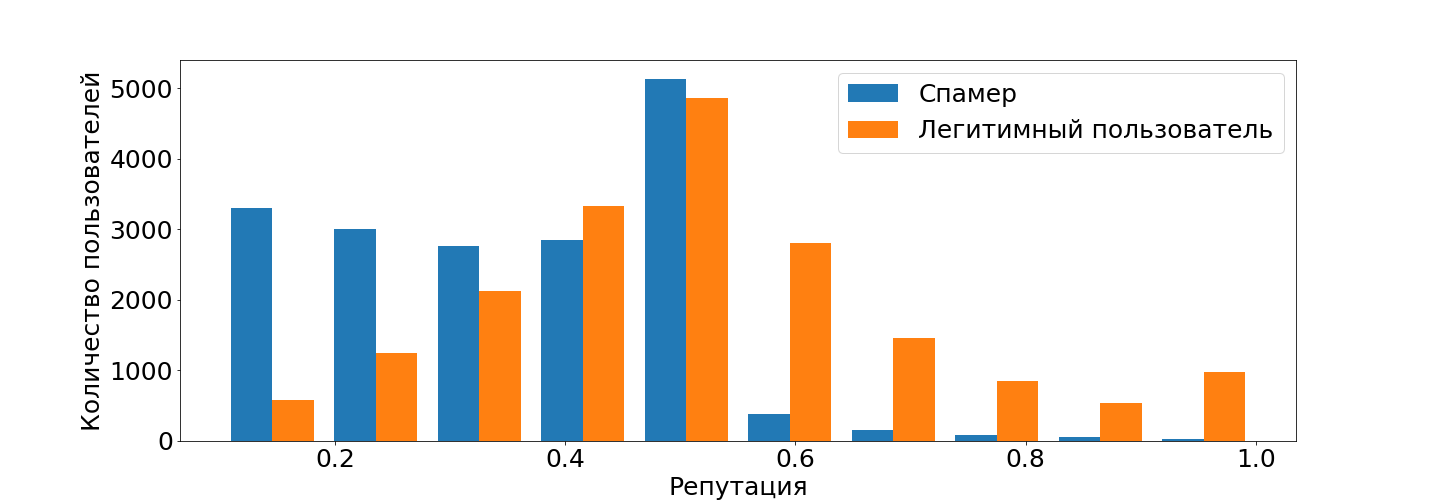
\includegraphics[width=1.0\textwidth]{pics/reputation}
    \caption{Распределение пользователей по репутации Twitter}
    \label{pic:reputation}
    \end{figure}

    \textbf{Признаки контента} фиксируют свойства текста каждого твита (табл. \ref{tab:features}).
     Среди 17 контентных атрибутов присутствует количество спам-слов и количество спам-слов на одно слово, которые генерируются путем сопоставления с известными спамовыми словами\footnote{https://github.com/splorp/wordpress-comment-blacklist/blob/master/blacklist.txt}.


     \begin{table}[H]
     \centering
     \resizebox{\textwidth}{!}{\begin{tabular}{|l|l|}
     \hline
     \textbf{Пользовательские признаки} & \textbf{Признаки контента}  \\
     \hline
     Длина названия профиля & Количество слов (КС) \\
     \hline
     Длина описания профиля & Количество символов \\
     \hline
     Количество подписок (ПС) & Количество пробелов \\
     \hline
     Количество подписчиков (ПЧ) & Количество слов с заглавной буквы (КЗ) \\
     \hline
     Количество твитов & КЗ/КС \\
     \hline
     <<Возраст>> аккаунта, ч. (ВА) &  Максимальная длина слова \\
     \hline
     Соотношение подписчиков и подписок (ПЧ/ПС) & Средняя длина слова \\
     \hline
     Репутация пользователь (ПЧ/(ПС + ПЧ)))  & Количество символов <<!>> \\
     \hline
     Прирост подписок (ПС/ВА) & Количество символов <<?>> \\
     \hline
     Количество твитов в день  & Количество URL (КЛ) \\
     \hline
     Количество твитов в неделю  & КЛ/КС \\
     \hline
      &  Количество хэштегов (КХ)\\
     \hline
      & КХ/КС \\
     \hline
      & Количество упоминаний (КУ) \\
     \hline
      & КУ/КС \\
     \hline
      & Количество спамовых слов (КСП) \\
     \hline
      & КСП / КС \\
     \hline
     \end{tabular}}

     \caption{Список итоговых признаков}
     \label{tab:features}
     \end{table}
  \end{subsection}

  \begin{subsection}{Используемые классификаторы}

    Наиболее популярным и эффективным подходом на данный момент является использование машинного обучения с учителем с различными признаками, основанными как на содержании сообщений, так и на свойствах отдельных профилей пользователей.

    Машинное обучение (machine learning) – это область научного знания, имеющая дело с алгоритмами, <<способными обучаться>>. Необходимость использования методов машинного обучения объясняется тем, что для многих сложных – <<интеллектуальных>> – задач (например, распознавание рукописного текста, речи и т. п.) очень сложно (или даже невозможно) разработать <<явный>> алгоритм их решения, однако часто можно научить компьютер обучиться решению этих задач. Одним из первых, кто использовал термин <<машинное обучение>>, был изобретатель первой самообучающейся компьютерной программы игры в шашки А. Л. Самуэль в 1959 г. \cite{Samuel}. Под обучением он понимал процесс, в результате которого компьютер способен показать поведение, которое в нее не было заложено <<явно>>. Это определение не выдерживает критики, так как не понятно, что означает наречие "явно". Более точное определение дал намного позже Т. М. Митчелл \cite{Mitchell}: говорят, что компьютерная программа обучается на основе опыта $E$ по отношению к некоторому классу задач $T$ и меры качества $P$, если качество решения задач из $T$, измеренное на основе $P$, улучшается с приобретением опыта $E$.

    В настоящее время машинное обучение имеет многочисленные сферы приложения, такие, как компьютерное зрение, распознавание речи, компьютерная лингвистика и обработка естественных языков, медицинская диагностика, биоинформатика, техническая диагностика, финансовые приложения, поиск и рубрикация текстов, интеллектуальные игры, экспертные системы и др.


    На этапе классификации и оценки были протестированы 5 алгоритмов, реализованных с использованием scikit-learn\footnote{http://scikit-learn.org/}: наивный байесовский классификатор (Naive Bayes classifier),
    метод \textit{k} ближайших соседей (\textit{k}-nearest neighbors algorithm, \textit{k}-NN)), метод опорных векторов (SVM), дерево принятия решений (Decision tree), случайные леса (Random forest).

    \begin{subsubsection}{Наивный байесовский классификатор}

Идея байесовский классификатора для спам-фильтра основана на предположении,
что некоторые слова особенно часто встречаются в спаме. Отсюда возникает идея посчитать для каждого слова $w$ из коллекции текстов количество сообщений с ним $n_{ws}$
в спаме (spam) и количесвто сообщений с ним $n_{wh}$ в <<не спаме>> (ham), а затем оценить вероятность появления каждого слова $w$ в спамном и неспамном тексте:

\begin{equation}
  P(w|spam) = n_{ws}/n_s; P(w|ham) = n_{wh}/n_s;
\end{equation}

Получив текст сообщения, для которого нужно определить, относится оно к спаму или нет, мы можем оценить вероятность появления всего текста в классе <<спам>> и в классе <<не спам>> произведением вероятностей слов:
\begin{equation}
P(text|spam) = P(w_1|spam)P(w_2|spam)...P(w_N|spam)
\end{equation}
\begin{equation}
P(text|ham) = P(w_1|ham)P(w_2|ham)...P(w_N|ham)
\end{equation}

<<Наивность>> подхода в этом случае состоит в предположении, что вхождение разных слов в текст – это независимые события.

Получив текст сообщения, для которого нужно определить, относится оно к спаму или нет, мы можем выбрать тот класс, в котором вероятность возникновения этого текста, домноженная на априорную вероятность класса, будет максимальна:
\begin{equation}
a(text) = arg⁡max_{y}⁡ P(y|text) = P(y) \times P(text|y)
\end{equation}

При этом важно понимать, что если новый текст содержит хотя бы одно слово, которое до этого не встречалось ни в одном из классов, то мы не сможем классифицировать текст как $spam$ или $ham$, поскольку $P(text|spam) = P(text|ham) = 0$.


В библиотеке sklearn наивный байесовский классификатор реализуется с помощью модуля sklearn.naive\_bayes\footnote{http://scikit-learn.org/stable/modules/naive\_bayes.html}.


\end{subsubsection}

    \begin{subsubsection}{Метод \textit{k} ближайших соседей}
      \label{alg:knn}
      Метод \textit{k} ближайших соседей (\textit{k} nearest-neighbor, \textit{k}-NN) относится к наиболее простым и в то же время универсальным методам, используемым как для решения задач классификации, так и восстановления регрессии. В случае классификации новый объект классифицируется путем отнесения его к классу, являющемуся преобладающим среди \textit{k} ближайших (в пространстве признаков) объектов из обучающей выборки. Если \textit{k} = 1, то новый объект относится к тому же классу, что и ближайший объект из обучающей выборки (см. Рис \ref{pic:knn1}, \ref{pic:knn2} ).

\begin{figure}[ht!]
\centering
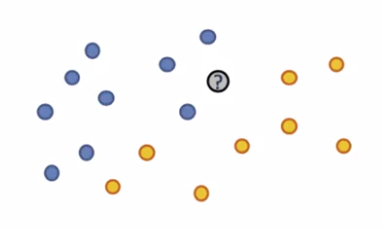
\includegraphics[width=0.4\textwidth]{pics/knn1}
\caption{Демонстрация метода \textit{k}-NN, \textit{k} = 1}
\label{pic:knn1}
\end{figure}


\begin{figure}[ht!]
\centering
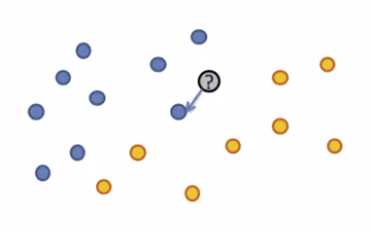
\includegraphics[width=0.4\textwidth]{pics/knn2}
\caption{Демонстрация метода \textit{k}-NN, \textit{k} = 1}
\label{pic:knn2}
\end{figure}

Можно модифицировать этот метод, поскольку принимать решения по одной точке может быть не очень надежно. Посмотрим на \textit{k} ближайших точек, выберем среди них доминирующий класс и отнесем новую точку к этому классу (cм. Рис \ref{pic:knn3} ).

\begin{figure}[ht!]
\centering
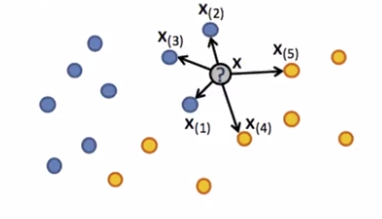
\includegraphics[width=0.4\textwidth]{pics/knn3}
\caption{Демонстрация метода \textit{k}-NN, \textit{k} = 5}
\label{pic:knn3}
\end{figure}




Также в алгоритм \textit{k}-NN можно добавить веса. Веса могут зависеть от номера соседа $w(x_{i} = w(i))$ или расстояния до соседа $w(x_{i} = w(d(x, x_{i})))$

Имея функцию весов можно определить класс как:

\begin{equation}
Z_{(1)} = w(x_{1}) + w(x_{2}) + ... + w(x_{m})
\end{equation}
\begin{equation}
Z_{(2)} = w(x_{m + 1}) + w(x_{m + 2}) + ... + w(x_{n})
\end{equation}
\begin{equation}
arg⁡max_Z Z_{(i)}
\end{equation}

Также можно классифицировать обьект посчитав центр обоих классов, как среднее арифметическое точек, которые входят в один и в другой класс (см. Рис \ref{pic:knn4}) и присвоить класс ближайшего центра новой точке:
\begin{equation}
\mu_{-1} = \frac{1}{l_{-1}} \sum\limits_{i: y_i = -1} x_i
\end{equation}

\begin{equation}
\mu_{+1} = \frac{1}{l_{+1}} \sum\limits_{i: y_i = +1} x_i
\end{equation}

\begin{figure}[ht!]
\centering
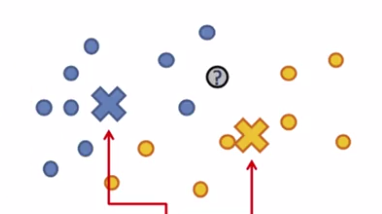
\includegraphics[width=0.4\textwidth]{pics/knn4}
\caption{Демонстрация метода \textit{k}-NN}
\label{pic:knn4}
\end{figure}

При решении задачи регрессии с помощью метода \textit{k}-NN  суммируются не просто веса обьектов, а веса, умноженные на значения функции, которую мы хотим приблизить, в этих объектах, нормировав ее на сумму всех весов.

В библиотеке sklearn метод \textit{k}-NN реализуется с помощью модуля sklearn.Neighbors\footnote{http://scikit-learn.org/stable/modules/neighbors.html}

\end{subsubsection}

    \begin{subsubsection}{Метод опорных векторов (SVM)}
	\label{svm}

Один из самых распространенных методов машинного обучения – машина опорных векторов (SVM – Support Vector Machine) – является развитием идей, предложенных в 1960–1970 гг. В. Н. Вапником и А. Я. Червоненкисом.
Данный метод представляет из себя линейный классификатор, использующий кусочно-линейную функцию потерь и L2-регуляризатор:

\begin{equation}
\sum\limits_{i=1}^l L(M_i) + \gamma ||w||^2 \rightarrow min_{w}
\end{equation}
где $L(M_i)$ - функция потерь, а $\gamma ||w||^2$ - регуляризатор

Идею метода удобно проиллюстрировать на следующем простом примере: даны точки на плоскости, разбитые на два класса (Рисунок \ref{pic:SVM1}).

  Проведем линию, разделяющую эти два класса. Далее, все новые точки (не из обучающей выборки) автоматически классифицируются следующим образом:
точка выше прямой попадает в класс A,
точка ниже прямой — в класс B.

\begin{figure}[ht!]
\centering
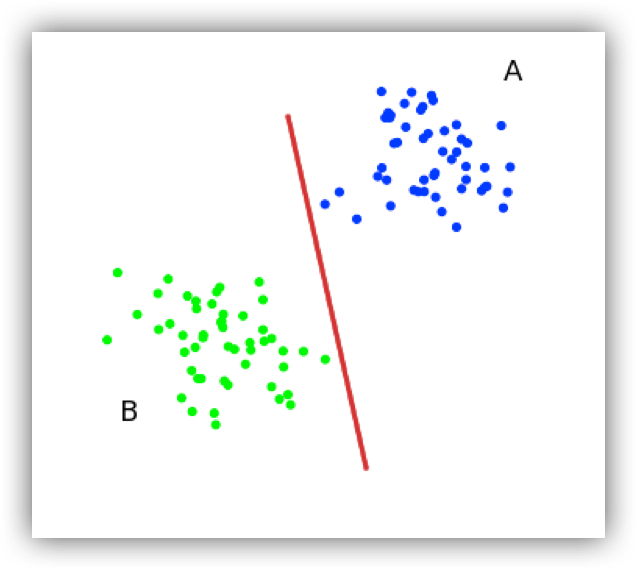
\includegraphics[width=0.4\textwidth]{pics/SVM1}
\caption{Демонстрация метода опорных векторов}
\label{pic:SVM1}
\end{figure}

Такую прямую назовем разделяющей прямой. Однако в пространствах высоких размерностей прямая уже не будет разделять наши классы, так как понятие «ниже прямой» или «выше прямой» теряет всякий смысл. Поэтому вместо прямых необходимо рассматривать гиперплоскости — пространства, размерность которых на единицу меньше, чем размерность исходного пространства. В $\mathbb{R}^3$, например, гиперплоскость — это обычная двумерная плоскость.
В нашем примере существует несколько прямых, разделяющих два класса (Рисунок \ref{pic:SVM2}):

\begin{figure}[ht!]
\centering
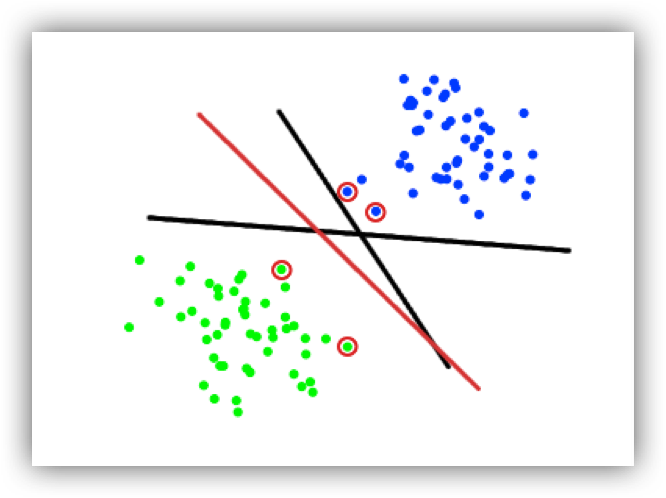
\includegraphics[width=0.4\textwidth]{pics/SVM2}
\caption{Демонстрация метода опорных векторов}
\label{pic:SVM2}
\end{figure}

С точки зрения точности классификации лучше всего выбрать прямую, расстояние от которой до каждого класса максимально. Другими словами, выберем ту прямую, которая разделяет классы наилучшим образом (красная прямая на рис. \ref{pic:SVM2}). Такая прямая, а в общем случае — гиперплоскость, называется оптимальной разделяющей гиперплоскостью.
Другими словами, оптимальной разделяющей гиперплоскостью называется гиперплоскость, ортогональная отрезку, соединяющему ближайшие точки выпуклых оболочек двух классов, и проходящая через середину этого отрезка.

Вектора, лежащие ближе всех к разделяющей гиперплоскости, называются \textit{опорными векторами} (support vectors). На Рисунке \ref{pic:SVM2} они помечены красными кружочками.

Для дальнейшей формализации положим в математической постановке задачи обучения с учителем,$\mathbb{Y} = \{-1,1\}, \mathbb{X} = \mathbb{R}^n$ .
Рассмотрим случай линейной разделимости. Пусть имеется обучающая выборка: $(x_1,y_1 ),…,(x_m,y_m ),x_i \in \mathbb{R}^n,y_i \in \{-1,1\}$.
Метод опорных векторов строит классифицирующую функцию  в виде
\begin{equation}
  f(x)=sign (w \times x + b)
\end{equation}
где $w \times x$ — скалярное произведение, $w$  — нормальный вектор к разделяющей гиперплоскости,$b$  — вспомогательный параметр. Те объекты, для которых $f(x) = 1$ попадают в один класс, а объекты с $f(x) = -1$ — в другой. Выбор именно такой функции неслучаен: любая гиперплоскость может быть задана в виде $w \times x + b = 0$ для некоторых $w$ и $b$.

Далее, мы хотим выбрать такие $w$ и $b$ которые максимизируют расстояние до каждого класса. Можно подсчитать, что данное расстояние равно $\frac{1}{||w||}$ (Рисунок \ref{pic:SVM3}) Проблема нахождения максимума $\frac{1}{||w||}$ эквивалентна проблеме нахождения минимума $||w||^2$. Запишем все это в виде задачи оптимизации:
\begin{equation}
  \begin{cases} arg⁡min_{(w,b)⁡} ||w||^2 , \\ y_i (w \times x+b) \geq 1, i=1,…,m \end{cases}
\end{equation}


которая является стандартной задачей квадратичного программирования и решается с помощью множителей Лагранжа.

\begin{figure}[ht!]
\centering
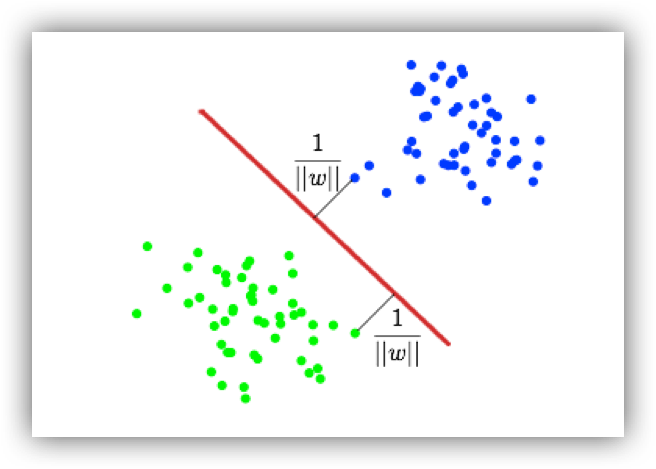
\includegraphics[width=0.4\textwidth]{pics/SVM3}
\caption{Демонстрация метода опорных векторов}
\label{pic:SVM3}
\end{figure}

На практике случаи, когда данные можно разделить гиперплоскостью, или, как еще говорят, \textit{линейно}, довольно редки. Пример линейной неразделимости можно видеть на Рисунок \ref{pic:SVM4}

\begin{figure}[ht!]
\centering
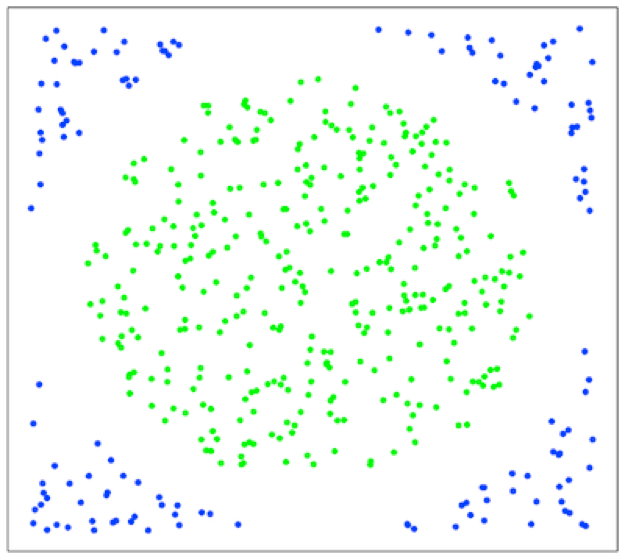
\includegraphics[width=0.4\textwidth]{pics/SVM4}
\caption{Демонстрация метода опорных векторов}
\label{pic:SVM4}
\end{figure}

В этом случае поступают так: все элементы обучающей выборки вкладываются в пространство $\mathbb{Z}$ более высокой размерности с помощью специального отображения $\varphi:\mathbb{R}^n \rightarrow Z$. При этом отображение  выбирается так, чтобы в новом пространстве $Z$ выборка была \textit{линейно} разделима.
Классифицирующая функция $f$ принимает вид
\begin{equation}
  f(x)=sign (w \times \varphi(x)+b)
\end{equation}
Выражение $K(x,x')= \varphi(x)\times \varphi(x')$ называется \textit{ядром} классификатора. С математической точки зрения ядром может служить любая положительно определенная симметричная функция двух переменных. Положительная определенность необходимо для того, чтобы соответствующая функция Лагранжа в задаче оптимизации была ограничена снизу, т.е. задача оптимизации была бы корректно определена. Точность классификатора зависит, в частности, от выбора ядра.
Чаще всего на практике встречаются следующие ядра:
\begin{enumerate}
  \item Полиномиальное: $K(x,x')= (x \times x'+ const)^d$
  \item Радиальная базисная функция: $K(x,x')= e^{-\gamma|x-x'|^2},\gamma > 0$
  \item Гауссова радиальная базисная функция: $K(x,x')= e^{-\frac{|x-x'|^2}{(2\sigma^2)}}$
  \item Сигмоид:$K(x,x') = \tanh⁡(k(x\times x')+c), k > 0, c < 0$
\end{enumerate}


Для того чтобы использовать метод опорных векторов для задачи классификации с числом классом $N > 2$, возможно также использовать следующие стратегии:
\begin{enumerate}
  \item "Каждый против каждого": построить $N(N-1)/2$ классификаторов на всех возможных подзадачах бинарной классификации. Новый объект классифицируется всеми построенными решающими правилами, затем выбирается преобладающий класс.
  \item "Один против всех": обучить $N$ моделей на задачах бинарной классификации вида "один класс против всех остальных". Класс нового объекта выбирается по максимальному значению отступа.
\end{enumerate}

В библиотеке sklearn алгоритм SVM реализуется с помощью модуля sklearn.svm.SVC\footnote{http://scikit-learn.org/stable/modules/generated/sklearn.svm.SVC.html}.
    \end{subsubsection}

    \begin{subsubsection}{Метод решающего дерева}
	\label{dt}
Метод деревьев решений (decision trees) является одним из наиболее популярных методов решения задач классификации и прогнозирования. Иногда этот метод Data Mining также называют деревьями решающих правил, деревьями классификации и регрессии. Это семейство алгоритмов, которое очень сильно отличается от линейных моделей и в то же время занимает крайне важную роль в машинном обучениии.

Суть метода деревьев решений легко продемонстрировать на примере известной задачи определения судьбы пассажиров <<Титаника>> (см. Рис. \ref{pic:dt1})

\begin{figure}[ht!]
\centering
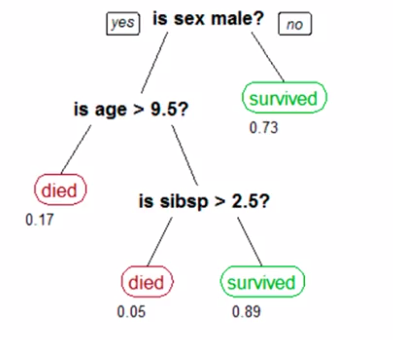
\includegraphics[width=0.4\textwidth]{pics/dt1}
\caption{Демонстрация метода деревьев решений}
\label{pic:dt1}
\end{figure}

 В первую очередь мы смотрим, какой пол у данного пассажира. Если это женщина, то мы сразу говорим, что она выживет, и этот ответ будет правильным в 73 \% случаев. Если это мужчина, то мы смотрим, сколько ему лет. Если девять или меньше, то мы перейдем в следующую ветку, а если больше девяти, то сразу говорим, что пассажир погиб. Если пассажиру меньше девяти лет, то мы смотрим, сколько родственников у этого пассажира было на борту. Если три или больше, то говорим, что он погиб. Если меньше, то говорим, что он выжил.

 В общем случае решающее дерево это некоторое бинарное дерево (не всегда), у которого в каждой внутренней вершине записано простое условие. В зависимости от того, верное оно или нет, мы будем идти либо вправо, либо влево от этой вершины. В каждом листе решающего дерева записан некоторый прогноз. Таким образом, мы берем некий объект, стартуем из корня и движемся по дереву, проверяя условие в текущей вершине. В зависимости от его выполнения идем либо влево, либо вправо. В конце концов мы попадаем в лист, в котором записан прогноз, который и выдается в качестве ответа модели.

 Можно строить и более сложные небинарные деревья, но, как правило, используются именно бинарные. Этого достаточно, чтобы решать большинство задач.


 Условия во внутренних вершинах также используются крайне простые. Наиболее частый вариант — проверка, находится ли значение j-того признака левее, чем некоторый порог $[x^j \leq t]$. То есть мы берем у объекта $j$-тый признак, сравниваем с порогом t, и если оно меньше порога, мы идем влево, если больше порога, мы идем вправо.


  Прогноз в листе будет вещественным, если это регрессия, и он будет пытаться как можно лучше приблизить истинный ответ. Если это классификация, то есть два варианта: дерево может выдавать либо номер класса (тогда в каждом листе будет записан просто тот или иной класс), либо распределение вероятности на классах. В этом случае в каждом листе будет записан некоторый вектор длины k, если k — это число классов, который будет говорить, насколько вероятно, что объект относится к тому или иному классу.

  Посмотрим, как выглядят зависимости, которые восстанавливают решающие деревья. Рассмотрим задачу классификации с двумя признаками. В ней три класса, и видно, что решающее дерево может очень неплохо отделить каждый класс от всех остальных (см. Рис. \ref{pic:dt2})


  \begin{figure}[ht!]
\centering
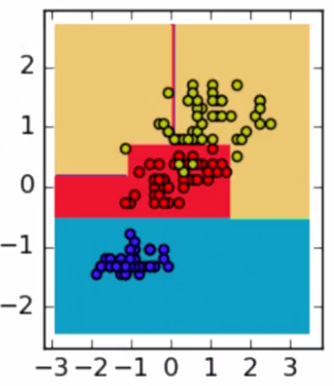
\includegraphics[width=0.4\textwidth]{pics/dt2}
\caption{Демонстрация метода деревьев решений}
\label{pic:dt2}
\end{figure}

  Видно, что разделяющая поверхность каждого класса кусочно-постоянная, и при этом каждая сторона разделяющей поверхности параллельна одной из осей координат из-за того, как именно мы выбрали условия. Каждое условие сравнивает значение ровно одного признака, ровно одной координаты с порогом.

  В то же время решающее дерево может легко переобучиться. Его можно сделать настолько глубоким, что каждый лист решающего дерева будет соответствовать ровно одному объекту обучающей выборки (см. Рис. \ref{pic:dt3}).

    \begin{figure}[ht!]
\centering
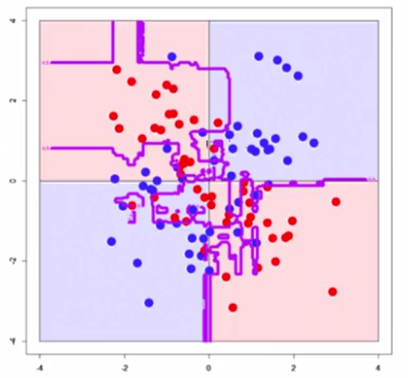
\includegraphics[width=0.4\textwidth]{pics/dt3}
\caption{Демонстрация метода деревьев решений}
\label{pic:dt3}
\end{figure}

   В этом случае, если мы запишем в каждом листе ответ соответствующего объекта, мы получим нулевую ошибку на обучающей выборке, но в то же время дерево будет явно переобученным.

  Поскольку дерево может достичь нулевой ошибки на обучающей выборке, нам не подходит любое дерево. Теоретически, каждую задачу можно решить деревом, которое будет иметь нулевую ошибку и при этом не быть переобученным, и, скорее всего, это будет минимальное дерево из всех, у которых нулевая ошибка. Минимальным оно может быть, например, в смысле количества листьев, то есть можно поставить задачу построить такое решающее дерево, которое не ошибается на данной выборке и при этом имеет меньше всего листьев. К сожалению, эта задача NP-полная, то есть ее невозможно решить за разумное время, поэтому в машинном обучении пользуются гораздо более простым подходом: строят дерево жадно, последовательно, от корня к листьям, а именно мы начинаем с пустого дерева, дальше выбираем каким-то образом корень, который разбивает нашу выборку на две, дальше разбиваем потомков этого корня и так далее. Ветвим дерево до тех пор, пока не решим, что этого достаточно. Пусть в вершине $m$ оказалась выборка $X_m$. Будем использовать некоторый критерий ошибки $Q$, который зависит от того, какие объекты попали в данную вершину, то есть $X_m$, и от параметров разбиения $j$ и $t$, то есть на основе какого признака мы разбиваем и с каким порогом мы сравниваем значение этого признака.


   Будем выбирать параметры $j$ и $t$-разбиения так, чтобы они минимизировали данный критерий ошибки $Q$. Подбирать параметр $j$ можно перебором, поскольку признаков у нас конечное число, а из всех возможных значений параметра $t$ (порога) можно рассматривать только те, при которых получаются различные разбиения. Можно показать, что этих значений $t$ столько, сколько различных значений признака $j$ на обучающей выборке. Например, можно отсортировать все значения $j$-того признака и брать пороги между этими значениями.

      \begin{equation}
	Q(X_m,j,t) \rightarrow min_{j,t}
  \end{equation}

   После того как мы выбрали конкретное разбиение, выбрали оптимальные значения параметров $j$ и $t$, мы разбиваем нашу вершину на две: левую и правую. При этом часть объектов, а именно те, на которых $j$-тый признак меньше или равен порогу $t$, отправляются влево (будем обозначать это подмножество как $X_l$), а часть объектов из $X_m$, те, у которых значение $j$-того признака больше порога $t$, отправляются вправо, и это подмножество обозначается как $X_r$:
         \begin{equation}
		X_l = {x \in X_m | [x^i \leq t ]}
  \end{equation}
           \begin{equation}
		X_r = {x \in X_m | [x^i > t ]}
  \end{equation}

   Эту процедуру можно повторить дальше для двух дочерних вершин, тем самым углубляя наше дерево.
   
   Процесс создания дерева происходит сверху вниз, т.е. является нисходящим. В ходе процесса алгоритм должен найти такой критерий расщепления, иногда также называемый критерием разбиения, чтобы разбить множество на подмножества, которые бы ассоциировались с данным узлом проверки. Каждый узел проверки должен быть помечен определенным атрибутом. Существует правило выбора атрибута: он должен разбивать исходное множество данных таким образом, чтобы объекты подмножеств, получаемых в результате этого разбиения, являлись представителями одного класса или же были максимально приближены к такому разбиению

Существуют различные критерии расщепления. Наиболее известные - мера энтропии и индекс Gini.

В некоторых методах для выбора атрибута расщепления используется так называемая мера информативности подпространств атрибутов, которая основывается на энтропийном подходе и известна под названием "мера информационного выигрыша" (information gain measure) или мера энтропии.

Другой критерий расщепления, предложенный Брейманом (Breiman) и др., реализован в алгоритме CART и называется индексом Gini. При помощи этого индекса атрибут выбирается на основании расстояний между распределениями классов.
Если дано множество $T$, включающее примеры из n классов, индекс Gini, т.е. $gini(T)$, определяется по формуле \ref{eq:gini}:
\begin{equation}
  \label{eq:gini}
  gini(T)=1 - \sum\limits_{i=1}^n p_i
\end{equation}
где $T$ - текущий узел, $p_i$ - вероятность класса $i$ в узле $p$, $n$  - количество классов.

   В какой-то момент нам все же придется остановиться. Критериев остановки очень много. Например, можно смотреть, сколько объектов находится в данной вершине. Если там всего один объект обучающей выборки, понятно, что дальше разбивать не имеет смысла; если же больше, можно разбивать дальше. Или, например, можно смотреть, какие объекты попали в эту вершину: если они все относятся к одному классу в задаче классификации, можно прекратить разбиение; если же есть несколько классов, можно разбивать дальше. Или, например, можно следить за глубиной дерева и останавливать разбиение, если глубина превышает некоторый порог, например, 10.

	Рассмотрим каким образом выбирать ответ в листе, если мы решили объявить вершину листом.  Если мы решаем задачу классификации, то наиболее логичным выбором будет возвращать тот класс, который наиболее популярен в выборке $X_m$, которая попала в данный лист. То есть для каждого класса $y$ мы считаем, сколько объектов этого класса попало в данную вершину, и возвращаем тот, который максимален:

	\begin{equation}
	a_m = arg⁡max_{y}  \sum\limits_{i \in X_m} [y_i = y]
	\end{equation}

	Если же мы хотим возвращать вероятности классов в данной вершине, это тоже очень легко сделать. Вероятность k-того класса оценивается как доля объектов k-того класса в данной вершине среди всех объектов, впавших в эту вершину, то есть среди всех объектов из $X_m$.

	\begin{equation}
	a_{mk} = \frac{1}{X_m}  \sum\limits_{i \in X_m} [y_i = k]
	\end{equation}

  В библиотеке sklearn алгоритм дерева решений реализуется с помощью модуля sklearn.trees\footnote{scikit-learn.org/stable/modules/tree.html}.
    \end{subsubsection}

    \begin{subsubsection}{Метод случайных лесов}
	\label{rf}
      Решающее дерево слишком легко подгоняется под обучающую выборку и получается непригодным для построения прогнозов. Бороться с переобучением довольно сложно. Надо либо использовать критерии остановок, которые слишком простые и не всегда помогают, либо делать стрижку деревьев, которая, наоборот, слишком сложная. Однако решающие деревья очень хорошо подходят для объединения в композиции, для построения одного непереобученного алгоритма на основе большого количества решающих деревьев. Композиция алгоритмов — это объединение $N$ алгоритмов в один. Алгоритм $a(x)$, который возвращает знак среднего (в случае задачи классификации) или просто среднее (в случае задачи регрессии) и называется композицией $n$ алгоритмов. А алгоритмы $b1, ..., bn$, которые мы объединяем в композицию, называются базовыми алгоритмами:

		\begin{equation}
		a(x) = sign \frac{1}{N}  \sum\limits_{n=1}^N b_n(x)
		\end{equation}

 Для того чтобы строить композицию, нужно обучить n базовых алгоритмов. При этом понятно, что нельзя их обучать на всей обучающей выборке. Они получатся одинаковыми, и в их усреднении не будет никакого смысла. Нужно делать их немного различными. Например, с помощью рандомизации, то есть обучать их по разным подвыборкам обучающей выборки. Поскольку решающие деревья очень сильно меняются даже при небольших изменениях обучающей выборки, такая рандомизация с помощью подвыборок будет очень хорошо влиять на их различность. Один из популярных подходов по построению подвыборок — это бутстрап. Предположим, что у нас есть полная обучающая выборка, состоящая из $l$ объектов. Мы генерируем из нее $l$ объектов с возвращением, то есть мы берем из нее некоторый случайный объект, записываем его в новую выборку и возвращаем обратно. То есть в какой-то момент мы можем снова его вытянуть и снова поместить в обучающую выборку. При этом новая выборка будет тоже иметь размер $l$, но при этом какие-то объекты будут в ней повторяться, а какие-то объекты исходной обучающей выборки не встретятся ни разу.  Можно показать, что количество различных объектов в бутстрапированной выборке будет равняться $0,632 \times l$, то есть примерно 63 \% объектов исходной выборки будет содержаться в бутстрапированной.

 Есть и другой подход к рандомизации. Это просто генерация случайного подмножества обучающей выборки. Например, мы берем случайные 50 \% объектов и на них обучаем базовый алгоритм. Этот подход чуть хуже, потому что в нем появляется гиперпараметр — размер подвыборки. В нашем примере это было 50 \%. В случае же с бутстрапом никаких параметром нет. Он без какой-либо настройки выдает нам подвыборку, что гораздо удобнее.

Среди достоинств алгоритма случайных деревьев можно выделить:
\begin{enumerate}
  \item высокое качество предсказания;
  \item способность эффективно обрабатывать данные с большим числом классов и признаков;
  \item внутреннюю оценку обобщающей способности модели;
  \item	легко построить параллельную высоко масштабируемую версию алгоритма;
  \item	метод обладает всеми преимуществами деревьев решений, в том числе
  o	отсутствием необходимости предобработки входных данных, обработкой как вещественных, так и категориальных признаков,
  o	поддержкой работы с отсутствующими значениями.

  К недостаткам можно отнести:
  \item	склонность к переобучению на некоторых задачах, особенно на зашумленных задачах;
  \item	большой размер получающихся моделей. Требуется  памяти для хранения модели, где  — число деревьев.
\end{enumerate}

В библиотеке sklearn модели «случайный лес»  реализуются с помощью модуля sklearn.ensemble\footnote{http://scikit-learn.org/stable/modules/ensemble.html}.
    \end{subsubsection}

  \end{subsection}

\end{section}
